\documentclass[12pt, a4paper]{article}

\usepackage[utf8]{inputenc}
\usepackage{lmodern}
%\usepackage{fourier}
\usepackage{setspace}
	\singlespacing

\usepackage[frenchb]{babel}
\usepackage{xspace}
\usepackage[margin= 2.5cm]{geometry}
\pagestyle{plain}
\renewcommand{\thefootnote}{\fnsymbol{footnote}}

\usepackage{tikz}
	\usetikzlibrary{shapes}
\usepackage{graphicx}
	\graphicspath{{img/}}

\usepackage{varioref}
	\renewcommand{\reftextbefore}{page précédente}
	\renewcommand{\reftextfacebefore}{page ci-contre}
	\renewcommand{\reftextafter}{page suivante}
	\renewcommand{\reftextfaceafter}{page ci-contre}
	\renewcommand{\reftextcurrent}{}

\usepackage{amsmath, amsfonts}
\everymath{\displaystyle}


\newcommand{\espace}{\vspace{.8cm}}
\newcommand{\pg}{

}

%% REMPLIR
\usepackage[colorlinks=true, allcolors=blue, pdfborder={0 0 0}]{hyperref}
	\hypersetup{
		pdftitle={Floss Inra Open Source},
		pdfsubject={Rapport Floss Inra Open Source},
		pdfkeywords={Floss Inra Open Source, IARISS, rapport},
		pdfauthor={IARISS Team}
	}
\title{Défi Floss Inra Open Source}
\newcommand{\authors}{Florent}

%
\begin{document}

\author{
\includegraphics{../_img/iariss_team.png} \\ {\sffamily \href{http://iarissteam.me}{iarissteam.me}}}
\date{\today}

\maketitle{}

{\sffamily Ce rapport à pour but de détailler les différentes stratégies mise oeuvre par l'équipe IarissTeam lors de la Nuit de l'Info 2012.} 

\espace{}
Nous avons choisi de développer notre projet selon le modèle de la méthode agile (c'est-à-dire des tâches, une durée pour réaliser chaque tâche, affcter les tâches à des personnes en particulier,\ldots{}). Afin de faciliter la mise en place de cette méthode, nous nous aidons du site \href{http://www.agilezen.com/}{agilezen.com}, un outil gratuit permettant la mise en place de méthode agile.

Nous nous sommes divisé en 3 pôles : une équipe de développement principal (nommée \og{}Master\fg{} chargé du développement des applications; une équipe de développement secondaire (nommé\og{}Padawan\fg{}) chargé du développement des pages de description de membre, du blog,\ldots{} et enfin un pôle communication, chargé d'assurer la présence sur les réseaux sociaux, la mise à jour du contenu des différents sites Web mis en place pour la nuit de l'info (le tumblr (\href{http://lesjoiesdelanuit.tumblr.com/}{Les joies de la Nuit}), le live (\href{http://live.iarissteam.me/}{Live IarissTeam}), le compte à rebours (\href{http://iarissteam.me/}{Compteur IarissTeam}),\ldots{}), ainsi que la rédaction des rapports.

Le pôle communication est le pivot de l'équipe : c'est lui qui décide d'affecter les tâches, de l'organisation en général. Avant de prendre une décision, on en discute bien évidemment tous ensemble.

Après avoir pris connaissance du sujet, nous avons donc décidé de nous réunir et de discuter ensemble de quoi faire, comment le faire, sous quel forme,\ldots{} (en ce qui concerne le code en lui même, le dernier mot revient logiquement aux équipes de développement). Une fois lancé dans le développement des différents sites web/applications, nous faisons une pause toute les deux heures afin de faire le point, voir comment chacun avance, si nous sommes dans les temps (ce qu'on appelle, dans le cas de la méthode agile, des \og{}itérations\fg{}).

L'application pricipale est développée en PHP, et sera déployée sur un serveur Linux. Afin de partager les ressources et le code entre les différents membres de l'équipe nous avons eu recours au programme Git et au site (\href{https://github.com/}{GitHub}). Ces derniers nous permettent de partager facilement les ressources entre nous, tout en les laissant accessibles et en libre consultation.
Certains membres de l'équipe, développant en local, utilise le système de DropBox afin de partager les ressources entre eux, avant de les synchroniser à l'aide de GitHub pour en faire profiter tous les membres de l'équipe.

Nous utilisons le principe d'intégration continue (\href{http://fr.wikipedia.org/wiki/Int\%C3\%A9gration_continue}{Wikipédia Intégration Continue}), afin de vérifier que chaque modification du code source n'entraîne pas de régression dans l'application.

Le code source de l'application sera libre, sous licence Creative Common. Nous essayons d'utiliser, notamment pour les images, des ressources libre de droit. Quand elles ne le sont malheureusement pas, nous précisons alors la provenance de cette ressource (comme sur le tumblr (lesjoiesdelanuit.tumblr.com), en bas de page).

Concernant le choix des logiciels, nous laissons aux développeurs le choix d'utiliser les outils qu'ils souhaitent (NetBeans, Eclipse, Notepad++,\ldots{})

Au cours de cette nuit, nous avons testé des méthodes de développement d'application déjà éprouvé à mainte reprise. Nous avons pu que constater leur efficacité : les méthodes utilisées se sont parfaitement adaptées au concept de la Nuit de l'Info.

\espace{}
\section*{Notre application}
METTRE ICI LE LIEN VERS LES APPLICATIONS, BLOG, ET GITHUB !
\espace{}
\begin{center}
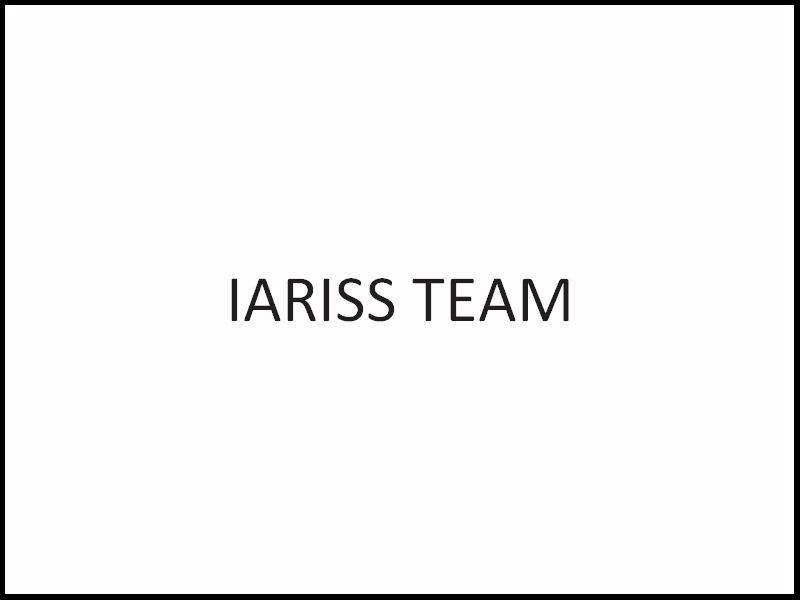
\includegraphics[width=.9\textwidth, keepaspectratio=true]{img/test.png}
\end{center}

\espace{}
\section*{Notre adresse postale}
	
IARISS
ENSISA Lumière
12 rue des Frères Lumière
68093 Mulhouse Cedex

%\espace{}
%\begin{figure}[h]
%	\begin{center}
%	\end{center}
%	\caption{\label{fig-} Légende}
%\end{figure}

\espace\vfill{}
Ce document a été rédigé en \LaTeX{} par \authors{} pour IarissTeam avec quelques tasses de café et beaucoup de bonne humeur.

Contactez-nous à \href{mailto:nuitinfo@iariss.com}{nuitinfo@iariss.com} pour tout renseignement supplémentaire !

\end{document}